\documentclass[a4paper,20pt]{article}

% Language setting
% Replace `english' with e.g. `spanish' to change the document language
\usepackage[fontset=ubuntu]{ctex}
% Set page size and margins
% Replace `letterpaper' with `a4paper' for UK/EU standard size
\usepackage[letterpaper,top=2cm,bottom=2cm,left=3cm,right=3cm,marginparwidth=1.75cm]{geometry}
\usepackage{placeins}
% Useful packages
\usepackage{amsmath}
\usepackage{graphicx}
\usepackage{tabto}
\usepackage[colorlinks=true, allcolors=blue]{hyperref}
\title{需求迭代过程}
\author{庄毅非\ 何迪\ 李予谦\ 应凌凯\ 刘奕骁}

\begin{document}
\maketitle


% 负责人:庄毅非(应用背景+业务机遇) 何迪(业务目标和成功标准,业务风险)
\section{需求变化概述}
这一部分主要是介绍在整个课程中,随着课程知识的学习和对项目要求的深入,我们对项目所包括的功能性需求和非功能性需求的整体理解的变化的一个概述,表现我们对需求变更进行管理的方式,如果想知道我们对每一个需求的详细理解的变化,请参考这份文档的第二部分\textbf{“需求迭代过程”}
\subsection{milestone 1 时期}
由于此时老师还没给出大概要做什么,所以我们小组再这时候有点漫无方向。通过查看和分析当前比较热门的开源项目分析平台ossinsight,我们大概总结了以下几个功能需求。
\begin{enumerate}
    \item 分析仓库总体信息,包括fork、stars等等
    \item 可视化仓库issue、pull、commit活动(主要是频率)随时间变化的情况
    \item 可视化社区贡献者变化
    \item 分析项目贡献者来自的国家,地区等
    \item 能够实现简单的用户管理功能,包括注册,登录等
    \item 用户应该能够实现收藏,点赞,评论等
    \item 用户应该能够进行仓库之间的对比
    \item 可视化项目代码行数随时间变化的情况
\end{enumerate}
\tab 这时候,我们对非功能需求的理解还不深刻,仅仅停留在界面美观、请求延迟小等浅显的层面。
\subsection{milestone 2、3以及workshop召开的时期}
在撰写 milestone 2 vision and scope 的时候,我们开始撰写项目应该具有的各种功能需求和非功能需求。这时候,我们对第一阶段列出的各种功能需求进行了进一步明确(因为之前的提出各种需求都比较浅显和模糊,都还不够明确)。
\begin{enumerate}
    \item 对仓库活动的可视化,应该能够支持多种图表类型(折线图、饼图等),也应该可以支持按天、月、年进行显示
    \item 对社区贡献者的分析,这时候我们认为应该统计的是项目的top10贡献者
    \item 对公司占比的显示,应该能够支持气泡图、词云等多种可视化方案
\end{enumerate}
\tab 我们也新增了下列非功能需求
\begin{enumerate}
    \item 性能需求
    \begin{enumerate}
        \item 能够对数据进行高效快速的爬取和存储
        \item 响应时间在3s以内
        \item 初次导入一个仓库在10min以内
        \item 初次计算一个仓库的信息在2min以内
    \end{enumerate} 
    \item 质量需求
    \begin{enumerate}
        \item 鲁棒性高
        \item 具有良好的扩展性
        \item 可维护性强
    \end{enumerate}
    \item 接口需求
    \begin{enumerate}
        \item 软件:我们选择linux发行版(支持centos、ubuntu)作为操作系统
        \item 硬件:2Core 4G 轻量应用服务器
    \end{enumerate}
\end{enumerate}

在参加了老师召开的workshop之后,我们重新列出了要实现的需求,也新增了一些需求(比如显示项目在特定时期内和设计相关的话题的分析等),按照紧急程度和重要性进行了优先级排序,结果如表所示。
\begin{table}[h]
\scalebox{0.8}{
\begin{tabular}{|l|l|l|l|l|}
\hline
编号       & 名称                                     & 紧急程度 & 重要性 & 优先级 \\ \hline
SE-UC-1  & 分析不同时期issue活动的频率的变化                    & 低    & 高   & 高   \\ \hline
SE-UC-2  & 分析不同时期pull活动的频率的变化                     & 低    & 高   & 高   \\ \hline
SE-UC-3  & 分析不同时期commit活动的频率的变化                   & 低    & 高   & 高   \\ \hline
SE-UC-4  & 分析不同时期issuer活动的频率的变化                   & 低    & 高   & 高   \\ \hline
SE-UC-5  & 分析不同时期puller活动的频率的变化                   & 低    & 高   & 高   \\ \hline
SE-UC-6  & 分析不同时期commiter活动的频率的变化                 & 低    & 高   & 高   \\ \hline
SE-UC-7  & 分析issue从提出到第⼀次得到response的平均时间变化        & 低    & 低   & 低   \\ \hline
SE-UC-8  & 分析issue从提出到closed所需要的平均时间变化            & 低    & 高   & 高   \\ \hline
SE-UC-9  & 界定出核⼼贡献者(28定律),统计数量,按照时间顺序显示在图表上       & 高    & 高   & 高   \\ \hline
SE-UC-10 & 显示核⼼贡献者背后的公司⽐例                         & 低    & 低   & 低   \\ \hline
SE-UC-11 & 将和设计有关的issue和pull分离出来                  & 高    & 高   & 高   \\ \hline
SE-UC-12 & 使⽤表格分析上述分理处来的issue和pull,绘制热门话题随时间变化的图表 & 高    & 高   & 高   \\ \hline
\end{tabular}
}
\end{table}

同时 我们在workshop之后也结合老师的要求,删去了部分无需实现的功能需求,比如用户注册、登录、收藏仓库等。我们也确定使用增量开发方式进行开发,对项目设立3个milestone,每一个milestone截止之前都设置了一定的多余时间进行缓冲,并且保证每一个milestone都尽量进行不少于2次的迭代,总的流程下来,开发还是比较顺畅的。



\subsection{项目开发过程中对需求理解的变化}
在项目开发过程中,我们也时刻注意对项目的需求进行管理,详细内容见下一个部分\textbf{“需求迭代过程”}

\section{需求迭代过程}
我们将根据具体的需求进行分类,来详细讲述我们对于具体的需求是如何进行迭代的。由于一些需求十分的相近,因此我们会将他们放在一起进行阐述。\par
注:SE-UC是 Software Engineering - Use Case 的缩写

\subsection{分析频率变化}
\subsubsection{原始需求}
SE-UC-1: 分析不同时期issue活动的频率的变化\par
SE-UC-2: 分析不同时期pull活动的频率的变化\par
SE-UC-3: 分析不同时期commit活动的频率的变化\par
SE-UC-4: 分析不同时期issuer活动的频率的变化\par
SE-UC-5: 分析不同时期puller活动的频率的变化\par
SE-UC-6: 分析不同时期commiter活动的频率的变化\par
\subsubsection{开发前的预想}
在实际的开发正式开始前我们已经发现,SE-UC-1~3已经在原先的代码中完成,因此我们选择基于原先的版本继续开发。我们准备使用曲线图,并提供可以更改展示的时间区间的方法。在设想中是准备使用顶部按钮组/Label来切换显示的时间格式(年月日)。
\subsubsection{最终的效果}
最终我们实现的效果依然选择了曲线图。由于使用顶部按钮组/Label有着无法选择具体时间段的局限性,我们改用了可以直接滑动窗口选择展示区域的底部时间选择栏(图中红色部分)。
\begin{figure}[h]
\centering
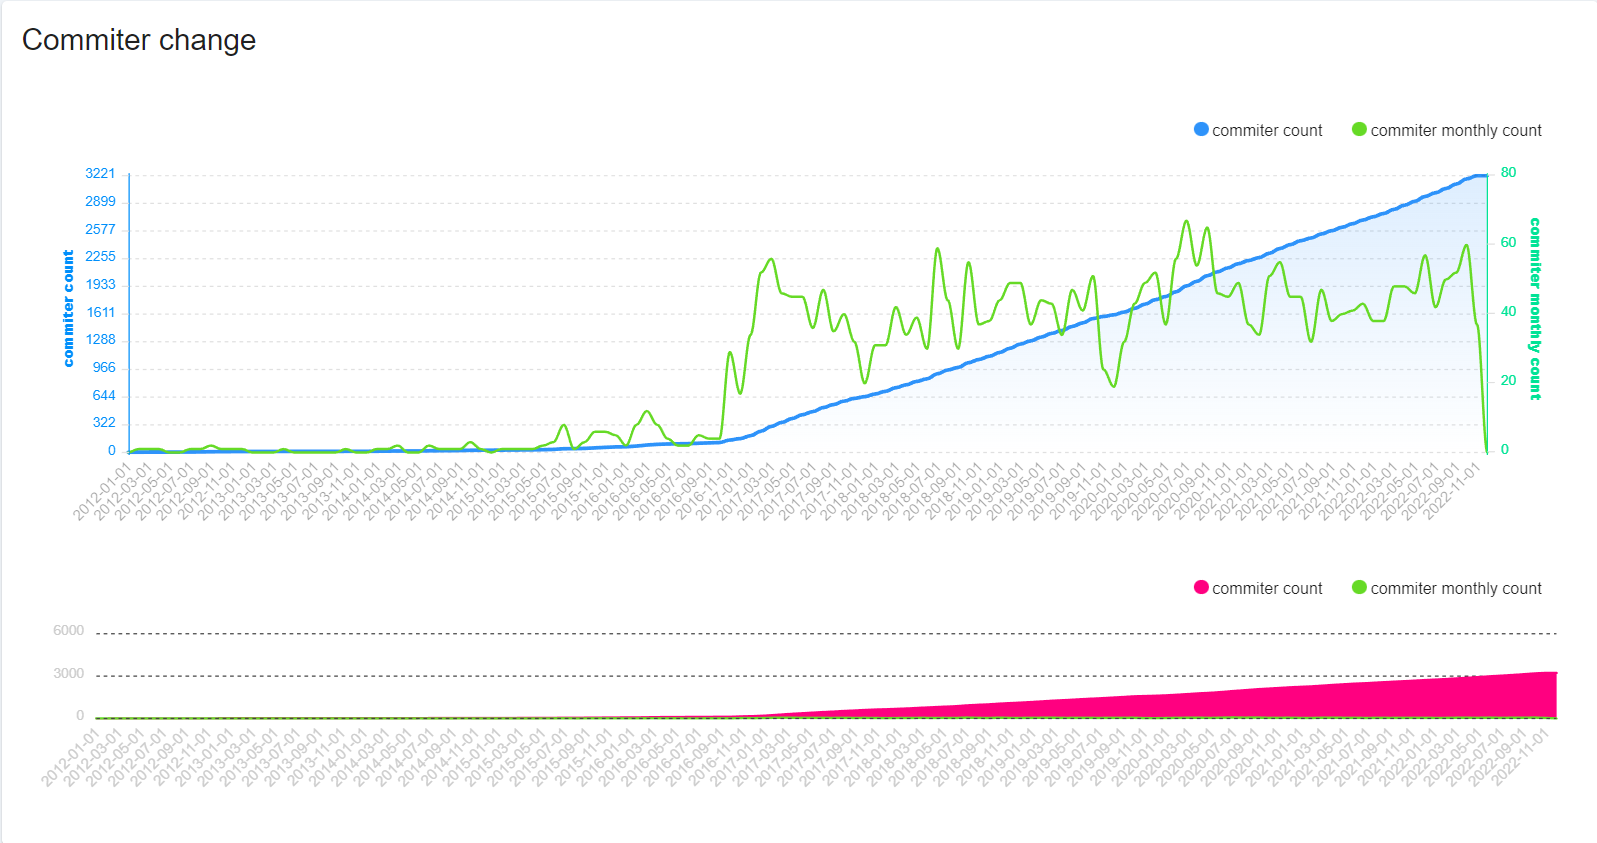
\includegraphics[scale=0.2]{pics/commiterChange.png}
\caption{commiter变化统计}
\label{fig:1}
\end{figure}



\subsection{统计issue时间变化}
\subsubsection{原始需求}
SE-UC-7: 分析issue从提出到第⼀次得到response的平均时间变化\par
SE-UC-8: 分析issue从提出到closed所需要的平均时间变化\par
\subsubsection{开发前的预想}
最初的开发中我们并没有一个明确的图表去合理的展示上述需求,在参考了OSS insight之后我们决定采用BOX graph来合理的表示每一个issue从提出到第⼀次得到response的时间。
\subsubsection{最终的效果}
最终我们依旧选择了BOX graph的表示方法,但对于数据处理上上作出了改变,由于计算每一个issues所需的时间资源消耗复杂,因此我们同样参考了OSS insight,展示对一段时间窗内的issue被response的平均时间。
\begin{figure}[h]
\centering
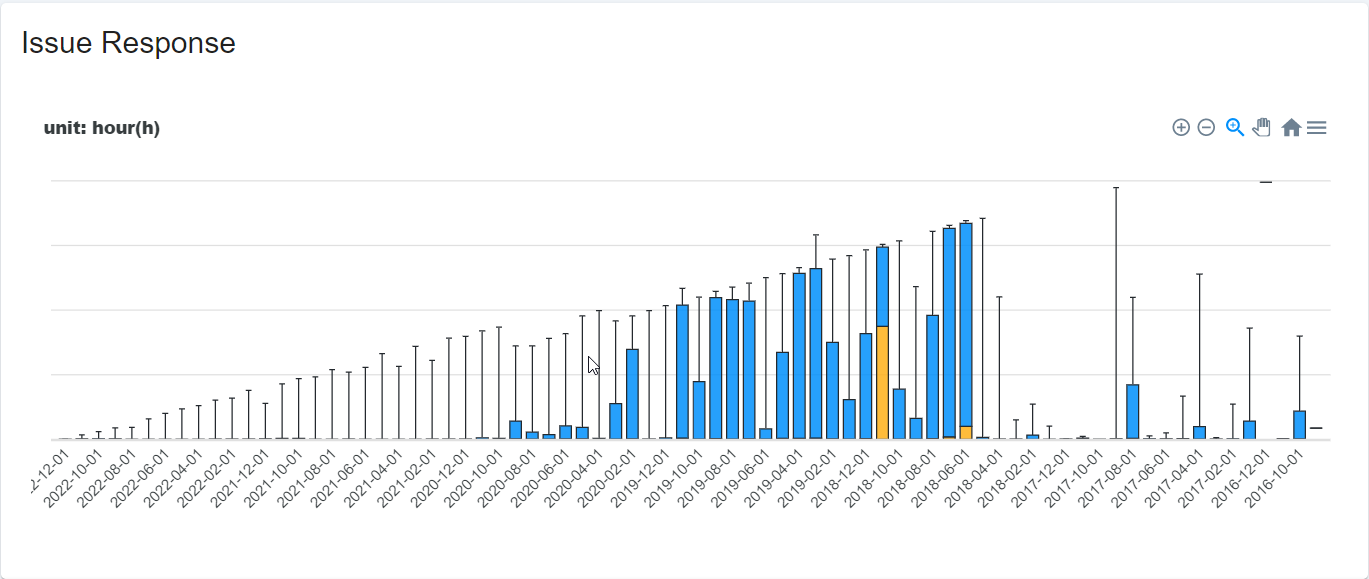
\includegraphics[scale=0.4]{pics/IsuueResponse.png}
\caption{issue从提出到第⼀次得到response的平均时间变化}
\label{fig:1}
\end{figure}


\subsection{界定并显示核心贡献者}
\subsubsection{原始需求}
SE-UC-9: 界定出核⼼贡献者(28定律),统计数量,按照时间顺序显示在图表上\par
\subsubsection{开发前的预想}
我们对核心贡献者的定义为:在一个时间段内,提交了该时间段内 80\% 的 commits 的贡献者们(按贡献次数降序排列,贡献次数多的优先计入,直到满 80\% 为止),将其计入核心贡献者。
我们预期采用折线图的方式对各个时期的核心贡献者进行统计。并给出一个列表进行对各个核心贡献者进行展示。
\subsubsection{最终的效果}
我们依照我们开发前的设想为核心贡献者绘制了折线图。考虑到我们的折线图是以年为单位展示的,因此其X轴会比较短,所以我们决定将折线图与核心贡献者列表放在同一行。而核心贡献者列表由上方的浮动按钮组以及下方的列表组成,下方列表的内容会根据上方按钮组的选择而动态切换。
\begin{figure}[h]
\centering
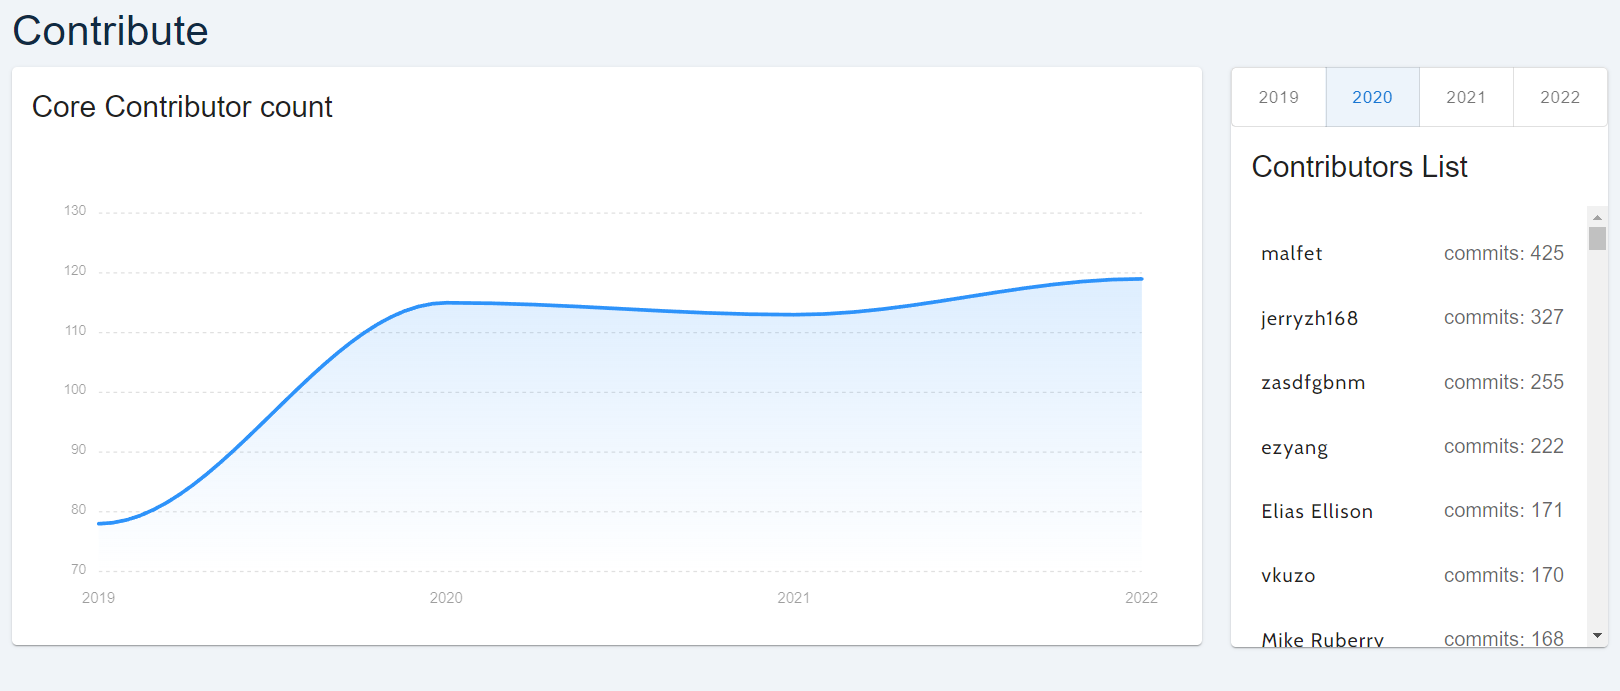
\includegraphics[scale=0.2]{pics/contributor.png}
\caption{commiter变化统计}
\label{fig:1}
\end{figure}

\subsection{显示核心贡献者公司}
\subsubsection{原始需求}
SE-UC-10: 显示核⼼贡献者背后的公司⽐例\par
\subsubsection{开发前的预想}
在我们完成对核心贡献者的界定与显示后,我们希望能够显示核心贡献者背后的公司比例,即从贡献者的比例显示转变到对于公司贡献占比的显示。
我们预期采用气泡图的方式对社区核⼼贡献者背后的公司⽐例进行统计,并通过对应气泡图的大小数量来对各个公司贡献占比进行展示。
\subsubsection{最终的效果}
我们依照我们开发前的设想为核心贡献者背后的公司比例绘制了气泡图。并且在这基础上我们将核心贡献者背后的公司依据贡献者本身拆分成若干数量且大小不一的气泡,优化了公司贡献占比的展示,方便了我们后续对公司与社区关系之间更好地分析。
\subsection{分离设计相关的话题}
\subsubsection{原始需求}
SE-UC-11: 将和设计有关的issue和pull分离出来(标准⾃洽即可)\par
\subsubsection{开发前的预想}
通过 NLP 或模糊搜索的方式,将 issue 和 pull request 根据不同的主题进行分类。由于 NLP 缺乏大量已经标记的数据集,并且我们在机器学习方面能力有限,所以打算采用模糊搜索的方式分离话题。
\subsubsection{最终的效果}
因为数据存储在 MongoDB 这样的 NoSQL 数据库中,并且我们期望模糊查询的能力不局限于 like "*key*" 的形式,所以采用了 ElasticSearch 作为数据的搜索引擎,实现了存储引擎和搜索引擎的分离。为了让搜索引擎能够及时获取存储引擎的更新,采用 mongo-connector,并开启 MongoDB 的副本模式,监听 MongoDB 的更新日志来同步到 ElasticSearch。\par
得益于 ElasticSearch 的倒排索引和强悍的全文计分模糊搜索机制,我们对不同话题预先设定好关键词集后,便可以从 ElasticSearch 中获取到任意时间段内的 issue 和 pull request 话题数量分布。\par
当然,这个结果也并不是精确的,通过对搜索出来的内容的观察,发现如 “测试” 话题设置了 “test” 关键词,但是许多主要目的并非测试,而是增加新功能/报告 bug 等的内容,因为也做了少量测试,涉及到 "test" 这个词而被包括进去。然而,判断一个 issue / pull request 的核心要义到底是什么而非断章取义,这脱离了模糊查询的能力范围,需要 NLP 和大量优秀数据的训练。但瑕不掩瑜的是,我们分离出来的话题内容总得来说已经具备较好的相关性。
\subsection{分析展示热门话题}
\subsubsection{原始需求}
SE-UC-12: 使⽤表格分析上述分理处来的issue和pull,绘制热⻔话题随时间变化的
图表\par
\subsubsection{开发前的预想}
并没有明确的展示方法,仅仅只是想要通过简单的表格或者词云图的形式将与设计相关的热门话题展示出来,并加以排序,但是这并没有很好的满足我们预想中能够展示社区活跃度这一预想要求。
\subsubsection{最终的效果}
最终我们为了突出社区的活跃度变化所以增加了时间轴,并且在这基础上通过饼图来更好的表示热门话题随时间的变化过程。通过不同时间热门话题不同的占比,我们就可以更好的观察社区中热门话题的变化情况。
\begin{figure}[h]
\centering
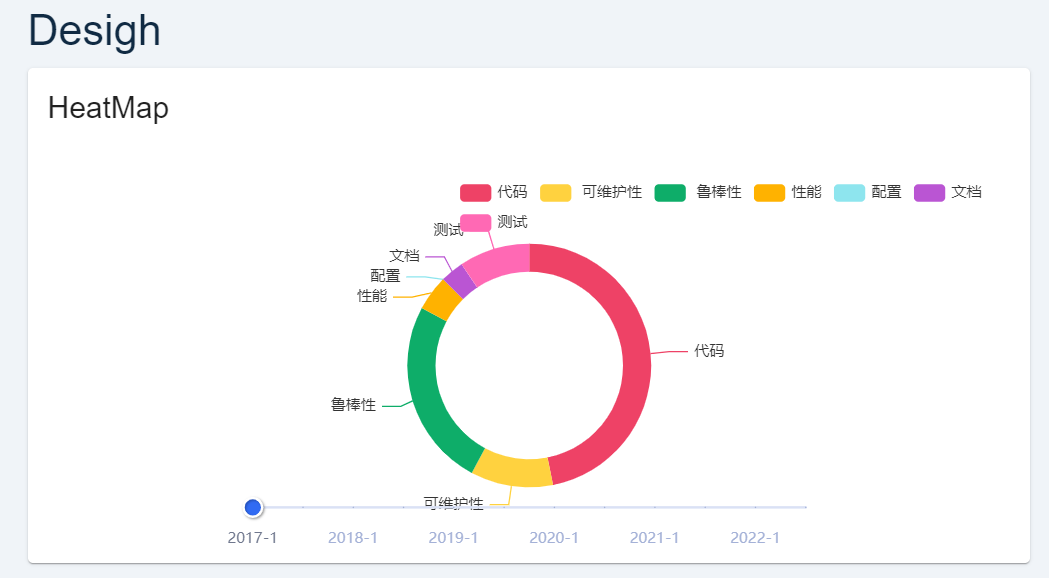
\includegraphics[scale=0.4]{pics/HeatMap.png}
\caption{分析展示热门话题}
\label{fig:1}
\end{figure}
\subsection{仓库对⽐}
\subsubsection{原始需求}
SE-UC-12: 仓库对⽐\par
\subsubsection{开发前的预想}
我们预期将在仓库的详情页面提供一个仓库对比的按钮,点下按钮之后就会弹出一个页面,可以选择对比的仓库,选择完成之后可以进入到一个仓库对比的数据展示。
而对比数据的展示方面,在我们预想中有两种思路,一种是直接使用文字对比的数据进行展示;另一种是选择和我们的主页面一样,将所有图表改成拥有两个系列的图表,在一张图上进行对比。
\subsubsection{最终的效果}
我们设计了如图中的仓库对比选择按钮,是采用了一个下拉框结合确认按钮的形式,并没有采用之前设想的弹出新窗口的设计。一是这种方案比较简单,二也是这样也相对比较整洁,很好地利用了之前的空余空间进行设计。
\begin{figure}[h]
\centering
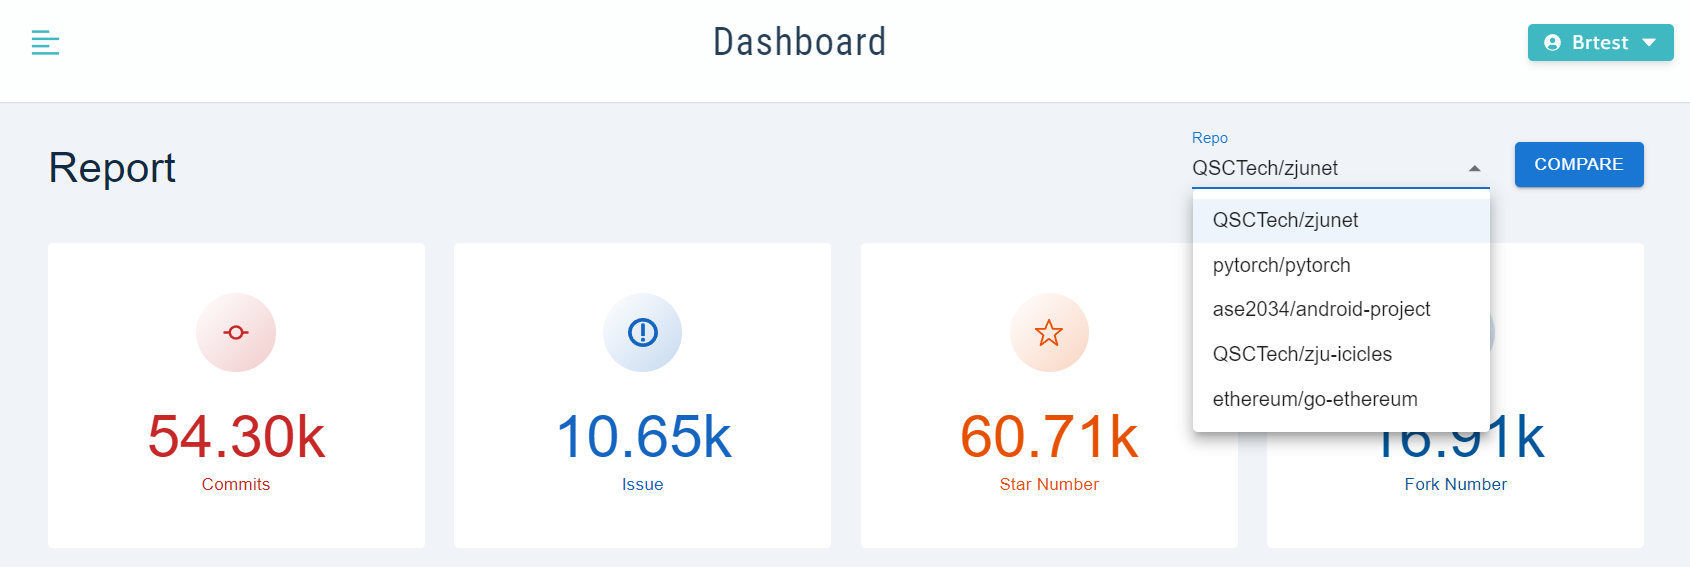
\includegraphics[scale=0.2]{pics/compare.png}
\caption{commiter变化统计}
\label{fig:1}
\end{figure}

我们在对比数据的展示方面并没有采取之前的两种思路,而是采用了第二种的改良版本。第一种思路过于简单,并不能达到较好的对比效果;而第二种思路看似比较美好,但是由于原本的图表已经比较复杂,有些图表中已经存在了不止一条曲线,如果再加上一个对比的仓库的数据,将会使整个图标的信息变得非常复杂,因此我们舍去了一些不重要的数据对比来简化整个功能。我们也在之前Compare按钮的同个地方放置了回到原先页面的按钮,使整个页面的风格统一。
我们仓库对比展示数据方面,参考了GitHub仓库对比工具 —— github-compare,通过对两个不同仓库之间commits,forks,stars,open issues等各项数据的对比,以方便每个仓库依次从以上各指标去其仓库首页看一下相关数据,进而更合理地衡量其稳定与否。
\begin{figure}[h]
\centering
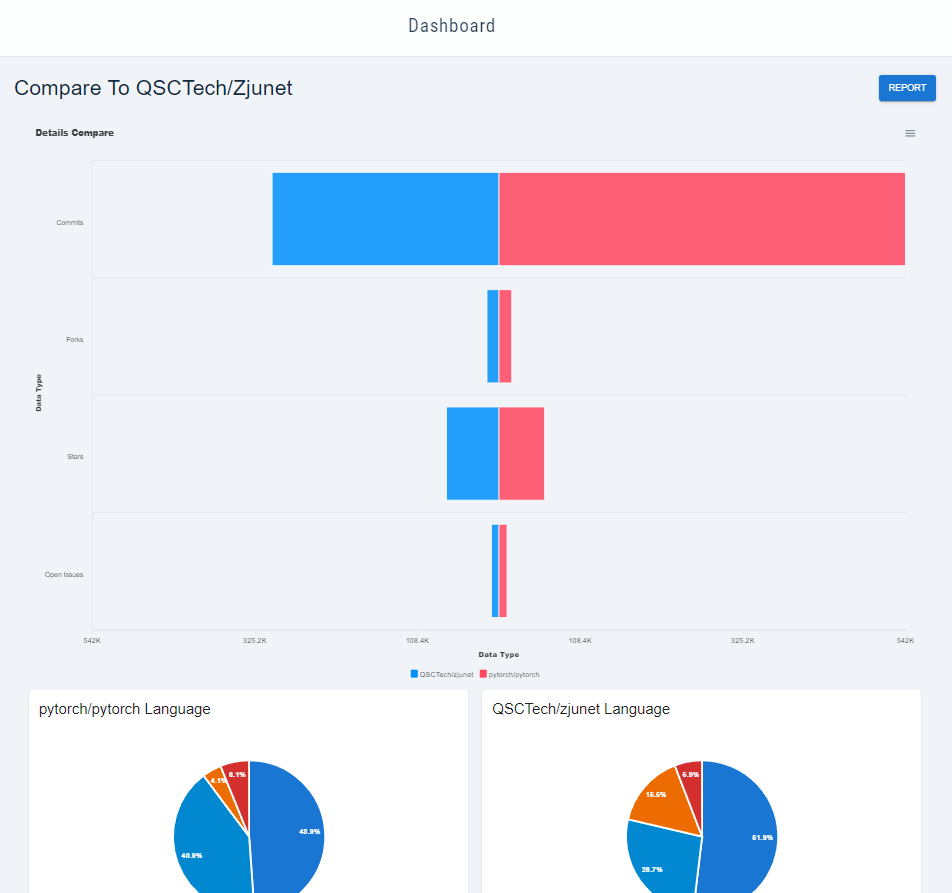
\includegraphics[scale=0.2]{pics/compareData.png}
\caption{commiter变化统计}
\label{fig:1}
\end{figure}
\end{document}